\documentclass{beamer}
%
% Choose how your presentation looks.
%
% For more themes, color themes and font themes, see:
% http://deic.uab.es/~iblanes/beamer_gallery/index_by_theme.html
%
\mode<presentation>
{
  \usetheme{default}      % or try Darmstadt, Madrid, Warsaw, ...
  \usecolortheme{default} % or try albatross, beaver, crane, ...
  \usefonttheme{default}  % or try serif, structurebold, ...
  \setbeamertemplate{navigation symbols}{}
  \setbeamertemplate{caption}[numbered]
} 

\usepackage[english]{babel}
\usepackage[utf8x]{inputenc}

\title[Data Mining]{Visualization-D3.js}
\author{Bingyu Wang}
\institute{Northeastern University}
\date{July 28, 2014}

\begin{document}

\begin{frame}
  \titlepage
\end{frame}

% Uncomment these lines for an automatically generated outline.
%\begin{frame}{Outline}
%  \tableofcontents
%\end{frame}

\section{Introduction}

\begin{frame}{Introduction}

\begin{itemize}
  \item Why d3.js? 
  \item Getting started
\end{itemize}

\end{frame}

\section{d3.js}

\subsection{Intro to d3.js}

\begin{frame}{Why d3.js?}

\begin{itemize}
	\item Most graphing packages take a configuration object.
	\item D3 is much more flexible and direct, and gets over the fact that the option you want are never available.
	\item Slower to get started but much more productive and flexible. 
	\item Great documentation, examples community.
\end{itemize}

% Commands to include a figure:
%\begin{figure}
%\includegraphics[width=\textwidth]{your-figure's-file-name}
%\caption{\label{fig:your-figure}Caption goes here.}
%\end{figure}

%\begin{table}
%\centering
%\begin{tabular}{l|r}
%Item & Quantity \\\hline
%Widgets & 42 \\
%Gadgets & 13
%\end{tabular}
%\caption{\label{tab:widgets}An example table.}
%\end{table}

\end{frame}

\begin{frame}{Fundamentals} 
Working with D3 requires an appreciation of the following concepts:

\begin{itemize}
	\item HTML 
	\item DOM
	\item CSS
	\item JavaScript
	\item SVG
\end{itemize}
\end{frame}

\begin{frame}{HTML}
Hypertext Markup Language is used to structure content for web browsers. The simplest HTML page looks like this:
\begin{figure}
\centering
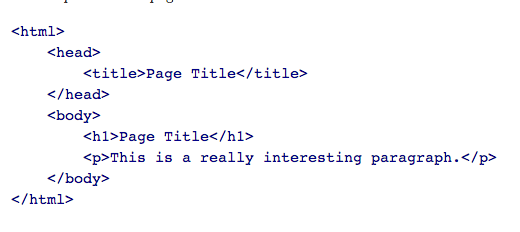
\includegraphics[width=1.0\textwidth]{./images/HTML.png}
\caption{\label{fig:samplemax} HTML}
\end{figure}
\end{frame}

\begin{frame}{DOM}
The Document Object Model refers to the hierarchical structure of HTML. Each bracketed tag is an element, and we refer to elements' relative relationships to each other in human terms: parent, child, sibling, ancestor, and descendant. In the HTML above, body is the parent element to both of its children, h1 and p (which are siblings to each other). All elements on the page are descendants of html.
\end{frame}

\begin{frame}{CSS}
Cascading Style Sheets are used to style the visual presentation of HTML pages.
\newline \\
D3 uses CSS-style selectors to identify elements on which to operate, so it is important to understand how to use them.
\end{frame}

\begin{frame}{JavaScript}
JavaScript is a dynamic scripting language that can instruct the browser to make changes to a page after it has already loaded.
\end{frame}

\begin{frame}{SVG}
D3 is at its best when rendering visuals as Scalable Vector Graphics. SVG is a text-based image format. Meaning, you can specify what an SVG image should look like by writing simple markup code, sort of like HTML tags. For example:
\begin{figure}
\centering
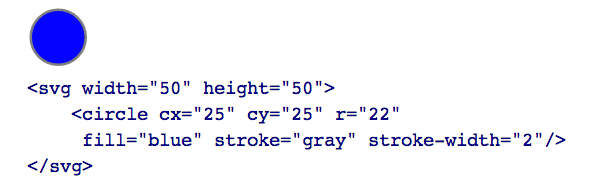
\includegraphics[width=1.0\textwidth]{./images/SVG.png}
\caption{\label{fig:samplemax} SVG}
\end{figure}

\end{frame}


\begin{frame}{Getting Started}
\begin{enumerate}
	\item Adding elements
	\item Binding data
\end{enumerate}
\end{frame}

\begin{frame}{Adding elements}
An example: \textbf{d3.select("body").append("p").text("New paragraph!");} \\
Let us walk through what just happened. In sequence, we:
\begin{enumerate}
	\item Invoked D3's select method, which selects a single element from the DOM using CSS selector syntax. (We selected the body.)
	\item Created a new p element and appended that to the end of our selection.
	\item Set the text content of that new, empty paragraph to New paragraph!
\end{enumerate} 
\end{frame}

\begin{frame}{Binding data}
Data visualization is a process of mapping data to visuals. Data in, visual properties out. \\
With D3, we bind our data input values to elements in the DOM. Binding is like attaching or associating data to specific elements, so that later you can reference those values to apply mapping rules.
\end{frame}

\subsection{Mathematics}

\begin{frame}{Readable Mathematics}

Let $X_1, X_2, \ldots, X_n$ be a sequence of independent and identically distributed random variables with $\text{E}[X_i] = \mu$ and $\text{Var}[X_i] = \sigma^2 < \infty$, and let
$$S_n = \frac{X_1 + X_2 + \cdots + X_n}{n}
      = \frac{1}{n}\sum_{i}^{n} X_i$$
denote their mean. Then as $n$ approaches infinity, the random variables $\sqrt{n}(S_n - \mu)$ converge in distribution to a normal $\mathcal{N}(0, \sigma^2)$.

\end{frame}

\end{document}
